% !TeX spellcheck = en_US
\documentclass[french]{yLectureNote}

\title{Mécanique}
\subtitle{Mécanique du point}
\author{Paulhenry Saux}
\date{\today}
\yLanguage{Français}

\professor{S.Deheuvels}%sebastien.deveuhels.irap.omp.eu

\usepackage{graphicx}%----pour mettre des images
\usepackage[utf8]{inputenc}%---encodage
\usepackage{geometry}%---pour modifier les tailles et mettre a4paper
%\usepackage{awesomebox}%---pour les boites d'exercices, de pbq et de croquis ---d\'esactiv\'e pour les TP de PC
\usepackage{tikz}%---pour deiffner + d\'ependance de chemfig
\usepackage{tkz-tab}
\usepackage{chemfig}%---pour deiffner formules chimiques
\usepackage{chemformula}%---pour les formules chimiques en \'equation : \ch{...}
\usepackage{tabularx}%---pour dimensionner automatiquement les tableaux avec variable X
\usepackage{awesomebox}%---Pour les boites info, danger et autres
\usepackage{menukeys}%---Pour deiffner les touches de Calculatrice
\usepackage{fancyhdr}%---pour les en-t\^ete personnalis\'ees
\usepackage{blindtext}%---pour les liens
\usepackage{hyperref}%---pour les liens (\`a mettre en dernier)
\usepackage{caption}%---pour la francisation de la l\'egende table vers Tableau
\usepackage{pifont}
\usepackage{array}%---pour les tableaux
\usepackage{lipsum}
\usepackage{yFlatTable}
\usepackage{multicol}
\newcommand{\Lim}[1]{\lim\limits_{\substack{#1}}\:}
\renewcommand{\vec}{\overrightarrow}
\newcommand{\norm}[1]{||\vec{#1}||}
\begin{document}

%\titleOne
\setcounter{chapter}{1}
	\chapter{Cinématique, forces, équilibre - Méthode}
	\section{Étude d'un mouvement en coordonnées cartésiennes dans une BOND}
\subsection{Déterminer la composante tangentielle de l'accélération}
\subsubsection{Création du vecteur unitaire tangent à la trajectoire}
On divise le vecteur vitesse par sa norme : $\vec{e_t} = \frac{\vec{v}}{\norm{v}}$.  La norme du vecteur vaut $\sqrt{v_x^2+v_y^2}$. Ainsi, \[\vec{e_t} = \frac{1}{\sqrt{v_x^2+v_y^2}} \begin{pmatrix}
 v_x\\v_y
\end{pmatrix} =  \begin{pmatrix}
 \frac{v_x}{\sqrt{v_x^2+v_y^2}}\\ \frac{v_y}{\sqrt{v_x^2+v_y^2}}
\end{pmatrix} \]
\subsubsection{Projection du vecteur accélération sur le vecteur crée}
On utilise la définition du produit scalaire avec les coordonnées (valable car nous sommes dans une BOND) : $\vec{B}\cdot \vec{A} =  x_ax_b+y_ay_b+z_az_b$

On projette donc $\vec{a}$ sur $\vec{e_t}$ : $a_t = a_xe_{t,x} + a_ye_{t,y} = a_x\frac{v_x}{\sqrt{v_x^2+v_y^2}} + a_y\frac{v_y}{\sqrt{v_x^2+v_y^2}}$.
\subsubsection{Déterminer la composante normale du vecteur accélération en connaissant sa norme et sa composante tangentielle}
On se trouve dans ce triangle rectangle :

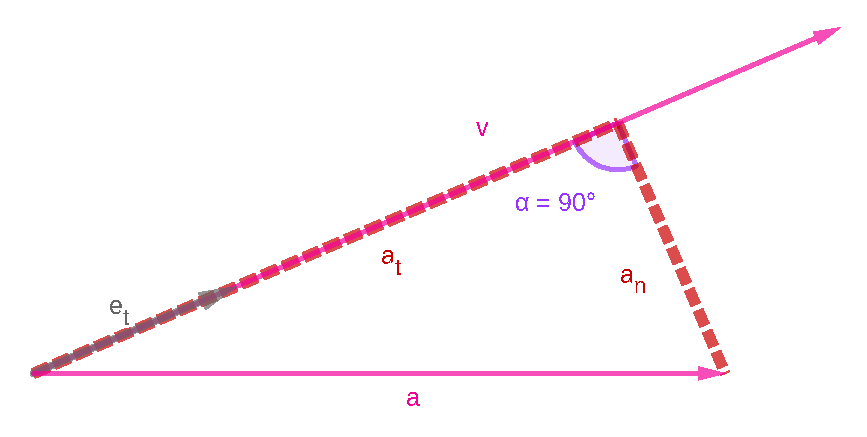
\includegraphics[scale=0.5]{rect30}

On peut donc appliquer le théorème de Pythagore :

\begin{flalign*}
\norm{a}^2 &= a_t^2 + a_n^2\\
a_n^2 &= \norm{a}^2 - a_t^2\\
a_n^2 &= \sqrt{a_x^2+a_y^2}^2 - a_t^2\\
a_n^2 &= a_x^2+a_y^2 - (a_x\frac{v_x}{\sqrt{v_x^2+v_y^2}} + a_y\frac{v_y}{\sqrt{v_x^2+v_y^2}})^2\\
a_n &= \sqrt{a_x^2+a_y^2 - (a_x\frac{v_x}{\sqrt{v_x^2+v_y^2}} + a_y\frac{v_y}{\sqrt{v_x^2+v_y^2}})^2}\\
\end{flalign*}
\end{document}

